\documentclass[dvipdfmx]{jsarticle}
\usepackage{mymacros}
\usepackage{amsmath,amssymb,amsthm}
\usepackage{tcolorbox,mathrsfs,multicol,subfiles}
\usepackage{tikz}
\usepackage[dvipdfmx]{hyperref}
\usepackage{pxjahyper}
\usetikzlibrary{cd}
\newtheorem{defi}{定義}[section]
\newtheorem{theo}[defi]{定理}
\newtheorem{lemm}[defi]{補題}
\newtheorem{corl}[defi]{系}
\newtheorem{prop}{命題}
\newtheorem{plob}{演習問題}
\newtheorem{axio}[defi]{公理}
\newtheorem{rem}[defi]{Rem}
\newtheorem{fact}[defi]{Fact}
\newtheorem{exam}[defi]{例}
\newtheorem{note}[defi]{Note}
\title{}
\author{}
\date{}
\begin{document}

\begin{prop}
  $G$加群 $M_1 , M_2 , M_3$に対して、 $C^n_i := C^n(G,M_i) , Z^n_i := Z^n(G,M_i) , B^n_i := B^n(G,M_i) , H^n_i := H^n(G,M_i)$と書くことにする。
  また、 $n$次コバウンダリー作用素 $\partial^n : C^n_i \longrightarrow C^{n+1}_i$を $\partial^n_i$と書くことにする。
  ここで以下のような行が完全列になっていてそれぞれ写像が可換な図を考える。
\begin{center}
  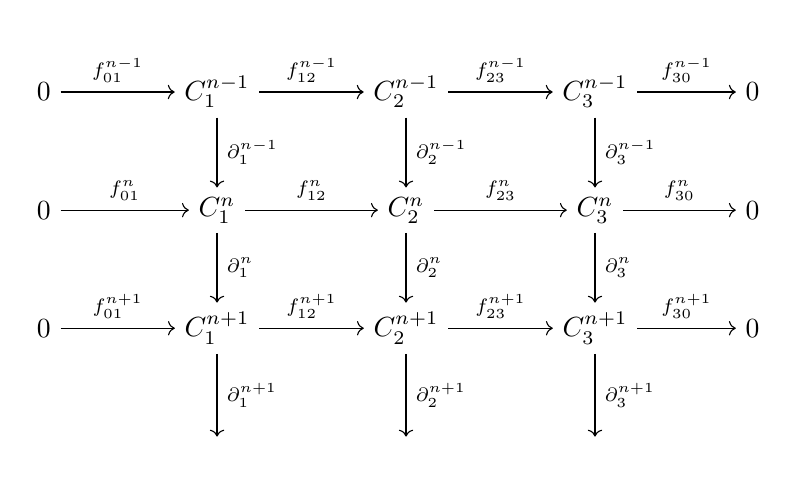
\begin{tikzpicture}[auto]
    %\draw [help lines] (0,0) grid (10,4);%(0,0)から(10,4)までの"細線の方眼"
    \node (hide) at (0,4.2) {};

    \node (0^{n-1}l) at (0,3.5) {$0$};
    \node (C^{n-1}_1) at (2.2,3.5) {$C^{n-1}_1$};
    \node (C^{n-1}_2) at (4.6,3.5) {$C^{n-1}_2$};
    \node (C^{n-1}_3) at (7,3.5) {$C^{n-1}_3$};
    \node (0^{n-1}r) at (9,3.5) {$0$};

    \node (0^nl) at (0,2) {$0$};
    \node (C^n_1) at (2.2,2) {$C^n_1$};
    \node (C^n_2) at (4.6,2) {$C^n_2$};
    \node (C^n_3) at (7,2) {$C^n_3$};
    \node (0^nr) at (9,2) {$0$};

    \node (0^{n+1}l) at (0,0.5) {$0$};
    \node (C^{n+1}_1) at (2.2,0.5) {$C^{n+1}_1$};
    \node (C^{n+1}_2) at (4.6,0.5) {$C^{n+1}_2$};
    \node (C^{n+1}_3) at (7,0.5) {$C^{n+1}_3$};
    \node (0^{n+1}r) at (9,0.5) {$0$};

    \node (0^{n+2}l) at (0,-1) {};
    \node (C^{n+2}_1) at (2.2,-1) {};
    \node (C^{n+2}_2) at (4.6,-1) {};
    \node (C^{n+2}_3) at (7,-1) {};
    \node (0^{n+2}r) at (9,-1) {};

    \draw[->] (0^{n-1}l) to node {$\scriptstyle f_{01}^{n-1}$} (C^{n-1}_1);
    \draw[->] (C^{n-1}_1) to node {$\scriptstyle f_{12}^{n-1}$} (C^{n-1}_2);
    \draw[->] (C^{n-1}_2) to node {$\scriptstyle f_{23}^{n-1}$} (C^{n-1}_3);
    \draw[->] (C^{n-1}_3) to node {$\scriptstyle f_{30}^{n-1}$} (0^{n-1}r);

    \draw[->] (0^nl) to node {$\scriptstyle f_{01}^n$} (C^n_1);
    \draw[->] (C^n_1) to node {$\scriptstyle f_{12}^n$} (C^n_2);
    \draw[->] (C^n_2) to node {$\scriptstyle f_{23}^n$} (C^n_3);
    \draw[->] (C^n_3) to node {$\scriptstyle f_{30}^n$} (0^nr);

    \draw[->] (0^{n+1}l) to node {$\scriptstyle f_{01}^{n+1}$} (C^{n+1}_1);
    \draw[->] (C^{n+1}_1) to node {$\scriptstyle f_{12}^{n+1}$} (C^{n+1}_2);
    \draw[->] (C^{n+1}_2) to node {$\scriptstyle f_{23}^{n+1}$} (C^{n+1}_3);
    \draw[->] (C^{n+1}_3) to node {$\scriptstyle f_{30}^{n+1}$} (0^{n+1}r);

    \draw[->] (C^{n-1}_1) to node {$\scriptstyle \partial^{n-1}_1$} (C^n_1);
    \draw[->] (C^{n-1}_2) to node {$\scriptstyle \partial^{n-1}_2$} (C^n_2);
    \draw[->] (C^{n-1}_3) to node {$\scriptstyle \partial^{n-1}_3$} (C^n_3);

    \draw[->] (C^n_1) to node {$\scriptstyle \partial^n_1$} (C^{n+1}_1);
    \draw[->] (C^n_2) to node {$\scriptstyle \partial^n_2$} (C^{n+1}_2);
    \draw[->] (C^n_3) to node {$\scriptstyle \partial^n_3$} (C^{n+1}_3);

    \draw[->] (C^{n+1}_1) to node {$\scriptstyle \partial^{n+1}_1$} (C^{n+2}_1);
    \draw[->] (C^{n+1}_2) to node {$\scriptstyle \partial^{n+1}_2$} (C^{n+2}_2);
    \draw[->] (C^{n+1}_3) to node {$\scriptstyle \partial^{n+1}_3$} (C^{n+2}_3);
  \end{tikzpicture}
\end{center}
このとき完全列であることから $f_{12}^i$は単射で $f_{23}^i$は全射である。
\begin{eqnarray*}
  \partial^* : H^n_3 & \longrightarrow & H^{n+1}_1 \\
  \overline{z} = z + B^n_3 & \longmapsto & \overline{x} = x + B^{n+1}_1 := \partial^*(\overline{z})
\end{eqnarray*}
で定まる準同型写像が存在することを示す。
\end{prop}

\begin{proof}
  $(1) \sim (4)$に分けて示す。
  ただし、より一般の完全列に対して $(1) \sim (3)$は蛇の補題から $\partial^* : \ker(\partial^n_3) = Z^n_3 \longrightarrow \coker(\partial^{n+1}_1) = C^{n+1}_1 / B^{n+1}_1$として境界準同型写像の存在性から示される。
  $(1)$では終域が $C^{n+1}_1$よりさらに $Z^{n+1}_1$に狭まることを、
  $(4)$ではとくに $H^n_3 \longrightarrow H^{n+1}_1$で定義できるようになることがさらに示される。

  $(1)$
  以下のような対応 $\partial^*_1$が存在すること
  \begin{eqnarray*}
    \partial^*_1 : Z^n_3 & \longrightarrow & Z^{n+1}_1 \\
    z & \longrightarrow & x
  \end{eqnarray*}
  証明では以下のように元を取っていく。
  \begin{center}
    \begin{tikzpicture}[auto]
      %\draw [help lines] (0,0) grid (10,4);
      \node (x) at (0,0) {$x := (f_{12}^{n+1})^{-1} \circ \partial^n_2(y)$};
      \node (partial^n_2y) at (3.5,0) {$\partial^n_2(y)$};
      \node (y) at (3.5,2) {$y := (f_{23}^n)^{-1}(z)$};
      \node (z) at (6,2) {$z$};
      \node (0r) at (6,0) {$0$};
      \node (0l) at (0,-2) {$0$};

      \draw[->] (z) to node {$\scriptstyle \partial^n_3$} (0r);
      \draw[->] (y) to node {$\scriptstyle f_{23}^n$} (z);
      \draw[->] (y) to node {$\scriptstyle \partial^n_2$} (partial^n_2y);
      \draw[->] (partial^n_2y) to node {$\scriptstyle f_{23}^{n+1}$} (0r);
      \draw[->] (x) to node {$\scriptstyle f_{12}^{n+1}$} (partial^n_2y);
      \draw[->] (x) to node {$\scriptstyle \partial^{n+1}_1$} (0l);
    \end{tikzpicture}
  \end{center}

  $z \in Z^n_3 = \ker(\partial^n) \subset C^n_3$をとる。
  このとき $f_{23}^n$は全射なので $f_{23}^n(y) = z$となる $y \in C^n_2$が少なくとも1つ存在する。
  このうちの一つを $y$としてとると $y = (f_{23}^n)^{-1}(z)$である。
  ここで図式が可換より $\partial^n_3 \circ f_{23}^n = f_{23}^{n+1} \circ \partial^n_2$なので
  $z \in \ker(\partial^n_3)$だから
  $\partial^n_3 \circ f_{23}^n(y) = \partial^n_3(z) = 0$
  なので $f_{23}^{n+1} \circ \partial^n_2(y) = 0$より $\partial^n_2(y) \in \ker(f_{23}^{n+1})$である。
  完全列であることから $\ker(f_{23}^{n+1}) = \im(f_{12}^{n+1})$と
  $f_{12}^{n+1}$は単射だからあるただ一つの $x \in C^{n+1}_1$が存在して
  $f_{12}^{n+1}(x) = \partial^n_2(y)$となるから
  この $x$により $\partial^*(z) := x = (f_{12}^{n+1})^{-1} \circ \partial^n_2 \circ (f_{23}^n)^{-1}(z)$として定めると
  $y = (f_{23}^n)^{-1}(z)$が一つに定まらないことより対応 $\partial^*_1 : Z^n_3 \longrightarrow C^{n+1}_1$が作られる。

  ここで $\partial^{n+1}_1(x) = \partial^{n+1}_1((f_{12}^{n+1})^{-1} \circ \partial^n_2(y))$である。
  図式が可換であることと $f_{12}^i$が単射だから $(f_{12}^{n+1})^{-1} \circ \partial^n_2 = \partial^n_1 \circ (f_{12}^n)^{-1}$より
  $\partial^{n+1} \circ \partial^n = 0$に注意すれば
  $\partial^{n+1}_1(x) = \partial^{n+1}_1((f_{12}^{n+1})^{-1} \circ \partial^n_2(y)) = \partial^{n+1}_1(\partial^n_1 \circ (f_{12}^n)^{-1}(y)) = (\partial^{n+1}_1 \circ \partial^n_1) \circ (f_{12}^n)^{-1}(y) = 0$
  となるから $x \in \ker(\partial^{n+1}_1) = Z^{n+1}_1$となる。
  したがって対応 $\partial^*_1$の終域は $Z^{n+1}_1$となるので上記のような対応が作られる。

  $(2)$
  対応 $\partial^*_1$から以下のような写像 $\partial^*_2$が作られること
  \begin{eqnarray*}
    \partial^*_2 : Z^n_3 & \longrightarrow & H^{n+1}_1 (:= Z^{n+1}_1 / B^{n+1}_1) \\
    z & \longrightarrow & \overline{\partial^*_1(z)} = \overline{x} = x + B^{n+1}_1
  \end{eqnarray*}
  いま $\partial^*_1$によって $z = z' \in Z^n_3$に対し、ある $y = (f_{23}^n)^{-1}(z) , y' = (f_{23}^n)^{-1}(z')$は $y \neq y'$になる可能性がある。
  その $y , y'$に対しては $\partial^n_2$が写像で $f_{12}^n$が単射より
  ただ一つの $x = (f_{12}^{n+1})^{-1} \circ \partial^n_2(y) , x' = (f_{12}^{n+1})^{-1} \circ \partial^n_2(y')$が存在する。
  このとき $x - x' \in B^{n+1}_1$であれば $\overline{x} = \overline{x'}$となるから $\partial^*_2$が写像になる。
  したがって $x - x' \in B^{n+1}_1$を示せばいい。

  以下のような可換性を用いる。
  \begin{center}
    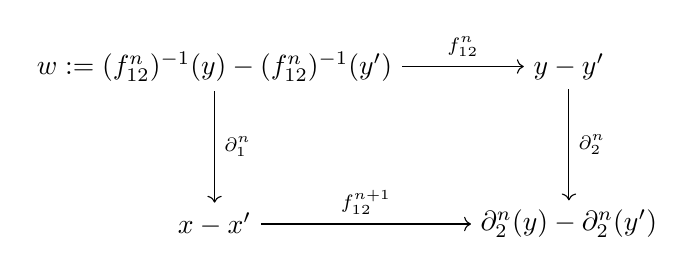
\begin{tikzpicture}[auto]
      %\draw [help lines] (0,0) grid (10,4);
      \node (x-x') at (0,0) {$x - x'$};
      \node (w) at (0,2) {$w := (f_{12}^n)^{-1}(y) - (f_{12}^n)^{-1}(y')$};
      \node (partial^n_2y - partial^n_2y') at (4.5,0) {$\partial^n_2(y) - \partial^n_2(y')$};
      \node (y-y') at (4.5,2) {$y - y'$};

      \draw[->] (y-y') to node {$\scriptstyle \partial^n_2$} (partial^n_2y - partial^n_2y');
      \draw[->] (w) to node {$\scriptstyle \partial^n_1$} (x-x');
      \draw[->] (x-x') to node {$\scriptstyle f_{12}^{n+1}$} (partial^n_2y - partial^n_2y');
      \draw[->] (w) to node {$\scriptstyle f_{12}^n$} (y-y');
    \end{tikzpicture}
  \end{center}

  $x - x' = (f_{12}^{n+1})^{-1} \circ \partial^n_2(y) - (f_{12}^{n+1})^{-1} \circ \partial^n_2(y')$である。
  $f_{12}^i$が単射で図式が可換より $(f_{12}^{n+1})^{-1} \circ \partial^n_2 = \partial^n_1 \circ (f_{12}^n)^{-1}$となる。
  よって $\partial^n_1$が準同型だから $x - x' = \partial^n_1 \circ (f_{12}^n)^{-1}(y) - \partial^n_1 \circ (f_{12}^n)^{-1}(y') = \partial^n_1((f_{12}^n)^{-1}(y) - (f_{12}^n)^{-1}(y'))$となる。
  ここで $w := (f_{12}^n)^{-1}(y) - (f_{12}^n)^{-1}(y') \in C^n_1$より
  $x - x' = \partial^n_1(w) \in \im(\partial^n_1) = B^{n+1}_1$より示された。

  とくに、以上のことから $\partial^*_2$は $y = (f_{23}^n)^{-1}(z)$のとり方によらないので以下ではある一つを任意に取ることとする。

  $(3)$
  写像$\partial^*_2$が準同型になること

  $\partial^*_2(z) = \overline{x} , \partial^*_2(z') = \overline{x'} , x = (f_{12}^{n+1})^{-1} \circ \partial^n_2(y) , x' = (f_{12}^{n+1})^{-1} \circ \partial^n_2(y')$とする。
  ここで $f_{23}^n$が準同型より
  $f_{23}^n(y + y') = f_{23}^n(y) + f_{23}^n(y') = z + z'$だから
  $y + y' = (f_{23}^n)^{-1}(z + z')$となる。
  また、 $f_{12}^{n+1} , \partial^n_2$が準同型より
  $f_{12}^{n+1}(x + x') = f_{12}^{n+1}(x) + f_{12}^{n+1}(x') = \partial^n_2(y) + \partial^n_2(y') = \partial^n_2(y + y')$なので
  $x + x' = (f_{12}^{n+1})^{-1} \circ \partial^n_2(y + y')$とできる。
  以上より $\partial^*_2(z + z') = \overline{x + x'} = x + x' + B^{n+1}_1 = (x + B^{n+1}_1) + (x' + B^{n+1}_1) = \overline{x} + \overline{x'} = \partial^*_2(z) + \partial^*_2(z')$となるから $\partial^*_2$は準同型になる。

  $(4)$
  準同型写像 $\partial^*_2$から以下のような準同型写像 $\partial^*$が誘導されること。
  \begin{eqnarray*}
    \partial^* : H^n_3 & \longrightarrow & H^{n+1}_1 \\
    \overline{z} = z + B^n_3 & \longmapsto & \partial^*_2(z) = \overline{x} = x + B^{n+1}_1
  \end{eqnarray*}
  以下のような可換性を用いる。
  \begin{center}
    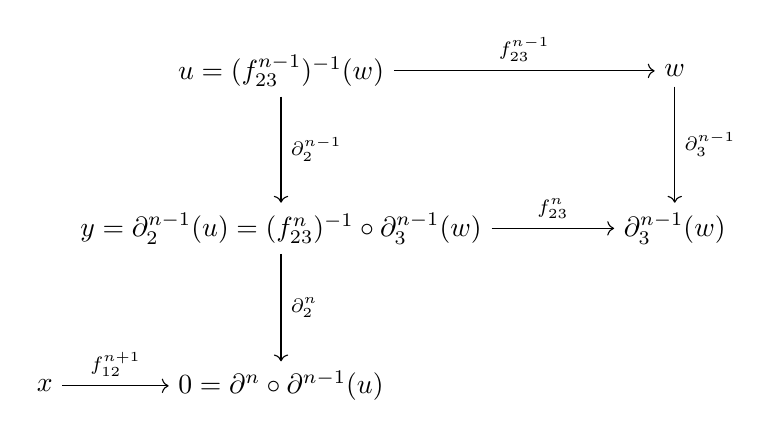
\begin{tikzpicture}[auto]
      %\draw [help lines] (0,0) grid (10,4);
      \node (x) at (0,0) {$x$};
      \node (y) at (3,2) {$y = \partial^{n-1}_2(u) = (f_{23}^n)^{-1} \circ \partial^{n-1}_3(w)$};
      \node (u) at (3,4) {$u = (f_{23}^{n-1})^{-1}(w)$};
      \node (w) at (8,4) {$w$};
      \node (partial^{n-1}_3w) at (8,2) {$\partial^{n-1}_3(w)$};
      \node (0) at (3,0) {$0 = \partial^n \circ \partial^{n-1}(u)$};

      \draw[->] (w) to node {$\scriptstyle \partial^{n-1}_3$} (partial^{n-1}_3w);
      \draw[->] (u) to node {$\scriptstyle f_{23}^{n-1}$} (w);
      \draw[->] (u) to node {$\scriptstyle \partial^{n-1}_2$} (y);
      \draw[->] (y) to node {$\scriptstyle f_{23}^n$} (partial^{n-1}_3w);
      \draw[->] (y) to node {$\scriptstyle \partial^n_2$} (0);
      \draw[->] (x) to node {$\scriptstyle f_{12}^{n+1}$} (0);
    \end{tikzpicture}
  \end{center}

  $\partial^*_2$はすでに準同型写像なので $\partial^*(\overline{z}) = \partial^*_2(z + B^n_3)$より $\partial^*_2(B^n_3) = 0$となれば
  $\partial^*(\overline{z}) = \partial^*_2(z) = \overline{x}$とできて準同型写像が誘導される。
  したがって $\partial^*_2(B^n_3) = 0$を示す。

  $B^n_3 = \im(\partial^{n-1}_3)$より $B^n_3$の元は
  任意の $w \in C^{n-1}_3$を用いて $\partial^{n-1}_3(w)$で書かれる。
  $\partial^n \circ \partial^{n-1} = 0$より $B^n_3 \im(\partial^{n-1}_3) \subset \ker(\partial^n_3) = Z^n_3$なので $\partial^*_2$の定義域に即している。
  この $\partial^{n-1}_3(w)$に対して今までと同様に
  $y = (f_{23}^n)^{-1}(\partial^{n-1}_3(w))$と
  $x = (f_{12}^{n+1})^{-1} \circ \partial^n_2(y)$が取れる。
  ここで $f_{23}^{n-1}$が全射なので $f_{23}^{n-1}(u) = w$となる $u \in C^{n-1}_2$が存在する。
  図式が可換より $\partial^{n-1}_3 \circ f_{23}^{n-1}(u) = f_{23}^n \circ \partial^{n-1}_2(u)$であるので
  $\partial^{n-1}_3(w) = f_{23}^n \circ \partial^{n-1}_2(u)$から
  $\partial^{n-1}_2(u) = (f_{23}^n)^{-1} \circ \partial^{n-1}_3(w) = y$
  となる。
  これより $\partial^n_2 \circ \partial^{n-1}_2 = 0$に注意すれば
  $\partial^*_2(\partial^{n-1}_3(w)) = (f_{12}^{n+1})^{-1} \circ \partial^n_2(y) = (f_{12}^{n+1})^{-1} \circ (\partial^n_2 \circ \partial^{n-1}_2)(u) = 0$
  となるので $\partial^{n-1}_3(w) \in \ker(\partial^*_2)$より
  $\partial^*_2(B^n_3) = 0$から適切に $\partial^*$が誘導される。

  以上より準同型写像 $\partial^* : H^n_3 \longrightarrow H^{n+1}_1 , \overline{z} \longmapsto \overline{x}$が存在することが示された。
\end{proof}

\end{document}
